\chapter{METODOLOGI}

% Ubah konten-konten berikut sesuai dengan isi dari metodologi

\section{Bahan dan peralatan yang digunakan}

Peralatan yang digunakan untuk penelitian ini antara lain:

\begin{enumerate}
  \item \textbf{GraspNet}, digunakan sebagai \emph{framework} robot lengan untuk
  melakukan tugas berupa \emph{autonomous grasping}. GraspNet sendiri adalah sebuah \emph{framework}
  berbasis \emph{deep learning} yang dirancang untuk melakukan prediksi \emph{pose grasping} secara akurat bagi lengan robot.
  \item \textbf{ROS}, yang mana merupakan sebuah \emph{framework}
  \emph{open-source} yang menyediakan kumpulan \emph{software}, \emph{library}, dan \emph{tools} untuk membantu pengembangan,
  pengendalian, serta komunikasi antar komponen dalam sistem robotik secara modular dan terdistribusi.
  \item \textbf{QT}, merupakan \emph{framework} pengembangan aplikasi \emph{cross-platform} yang berbasis C++,
  digunakan untuk membangun antarmuka grafis (GUI) dan aplikasi dengan performa tinggi serta kompatibilitas luas di berbagai sistem operasi.
  \item \textbf{Hardware}, Hardware yang digunakan dalam penelitian ini adalah robot quadruped dari DeepRobotics, Arm Robot custom dengan servo motor dynamixel,
  serta controller custom yang dikembangkan oleh tim robot Ichiro ITS.
\end{enumerate}

% \lipsum[11]
% % Contoh input gambar dengan format *.jpg
% \begin{figure} [H] \centering
%   % Nama dari file gambar yang diinputkan
%   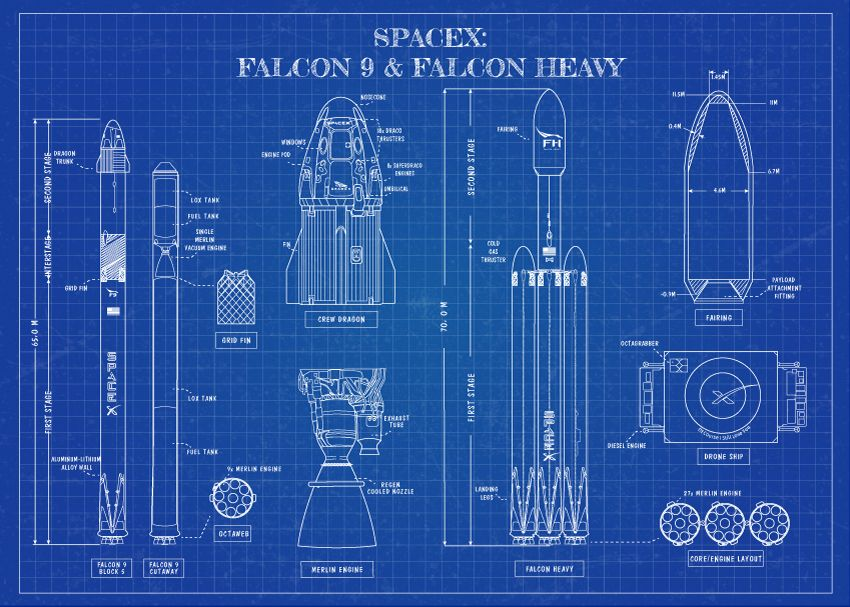
\includegraphics[scale=0.45]{gambar/blueprint.jpg}
%   % Keterangan gambar yang diinputkan
%   \caption{\emph{Blueprint} roket yang akan diuji coba \parencite{SpaceXBlueprint}}
%   % Label referensi dari gambar yang diinputkan
%   \label{fig:Blueprint}
% \end{figure}
% % Contoh penggunaan referensi dari gambar yang diinputkan
% Pada \emph{blueprint} yang tertera di Gambar \ref{fig:Blueprint}. \lipsum[12]

\section{Metode yang digunakan}

Metodologi yang digunakan pada penelitian ini terdiri dari beberapa tahapan seperti yang
ditunjukkan pada gambar berikut.

\begin{figure} [H] \centering
  % Nama dari file gambar yang diinputkan
  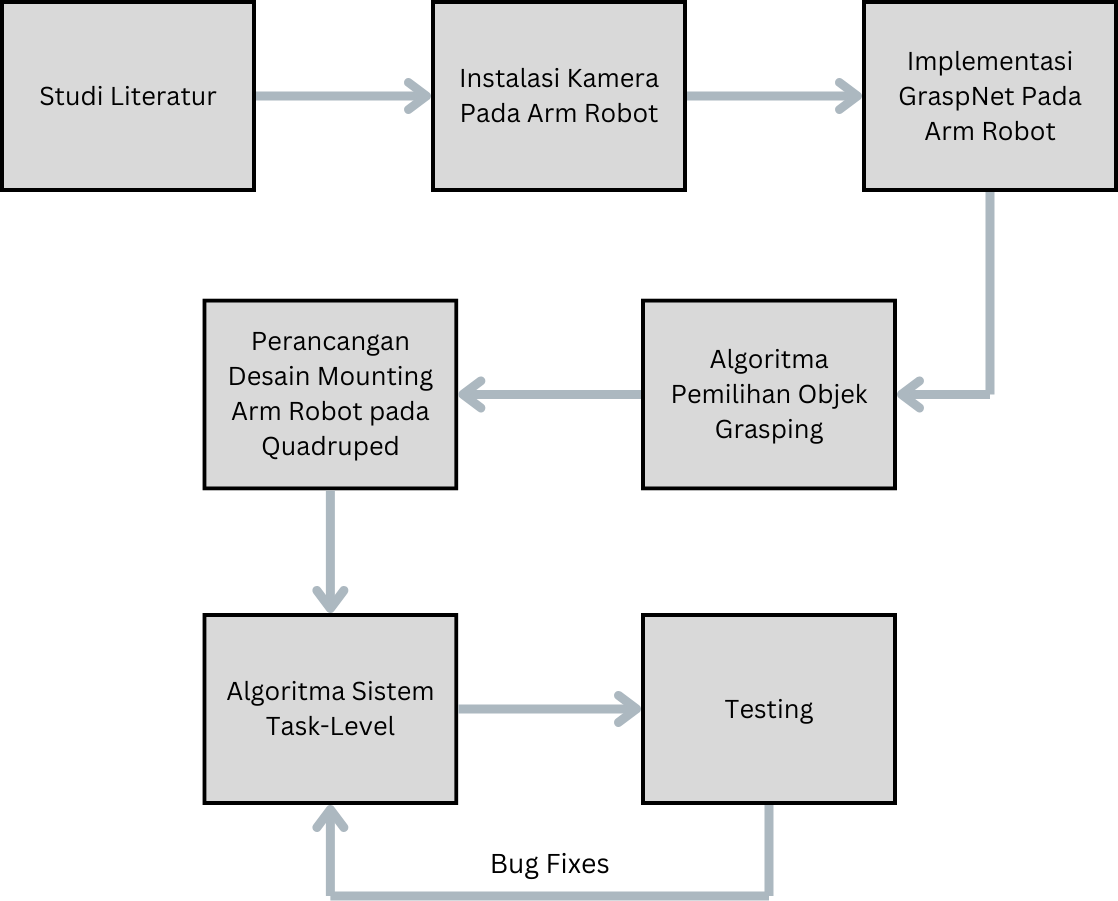
\includegraphics[scale=0.4]{gambar/Blok Diagram Metodologi.png}
  % Keterangan gambar yang diinputkan
  \caption{Blok Diagram Perancangan Penelitian}
  % Label referensi dari gambar yang diinputkan
  \label{fig:diagram_metode}
\end{figure}

